\chapter{Motor Learning in Virtual Reality}
\label{chapter:theoretical_background}
The aquisition and improvement of movements is called motor learning~\cite{mlbook}

\section{Motor Learning}
\label{section:motor_learning}
grundlagen des motor learning
\section{Visual Perspectives}
\label{section:visual_perspectives}
\begin{figure}[htb]
	\centering
	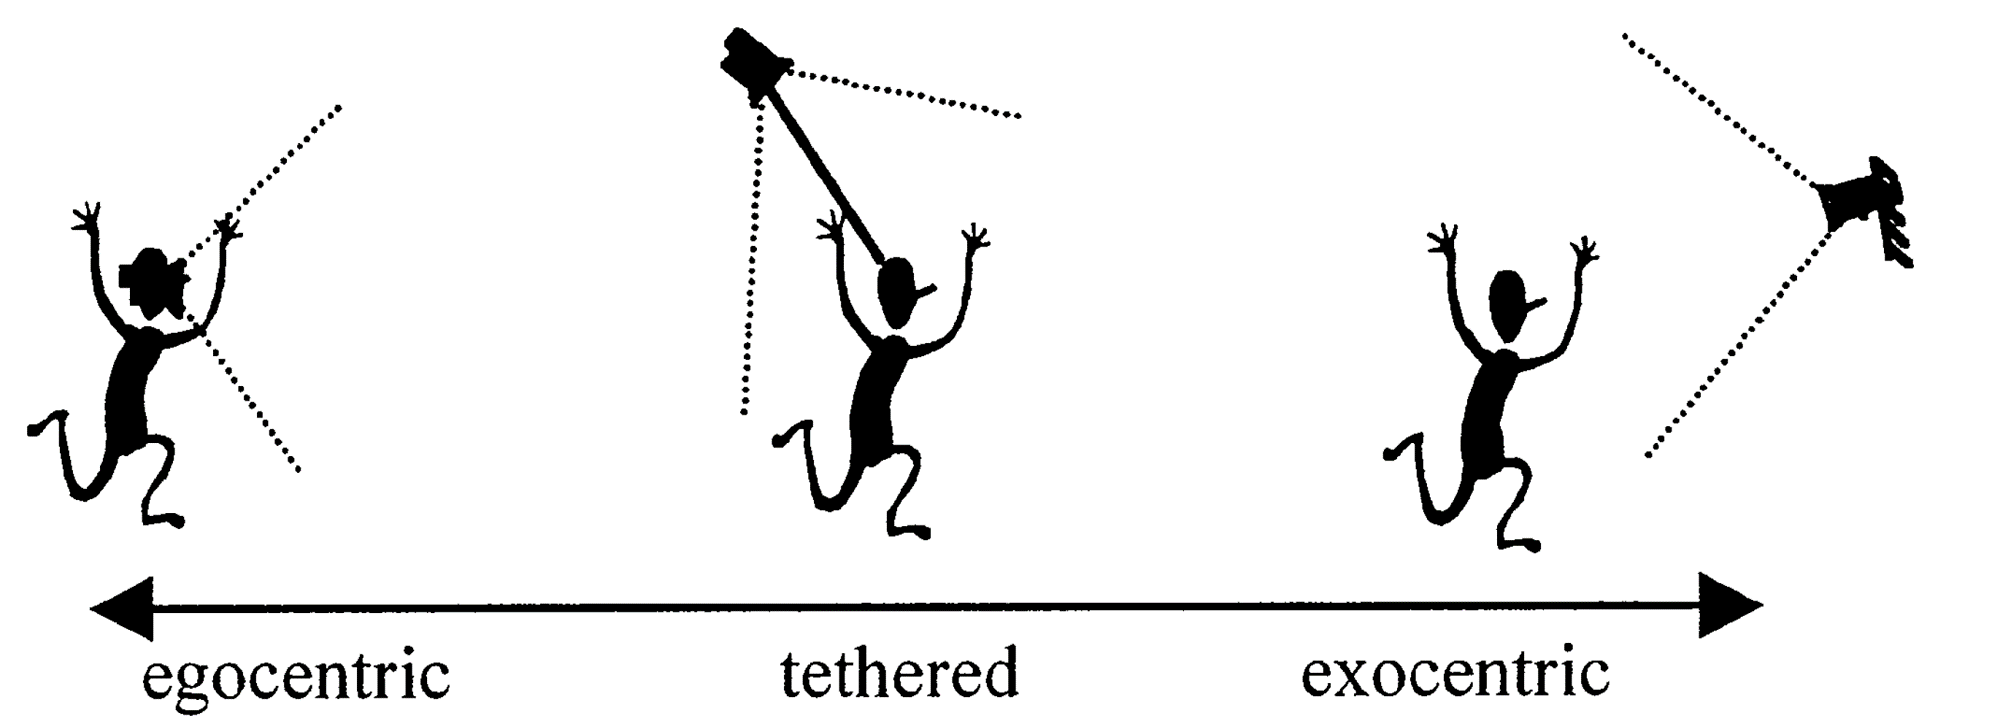
\includegraphics[width=\textwidth]{figures/ego_exo_continuum.PNG}
	\caption[Centricity continuum]{Centricity continuum by Wang and Milgram~\cite{centricitycontinuum}}
	\label{fig:ego-exo-continuum}
\end{figure}

\begin{figure}[htb]
	\centering
	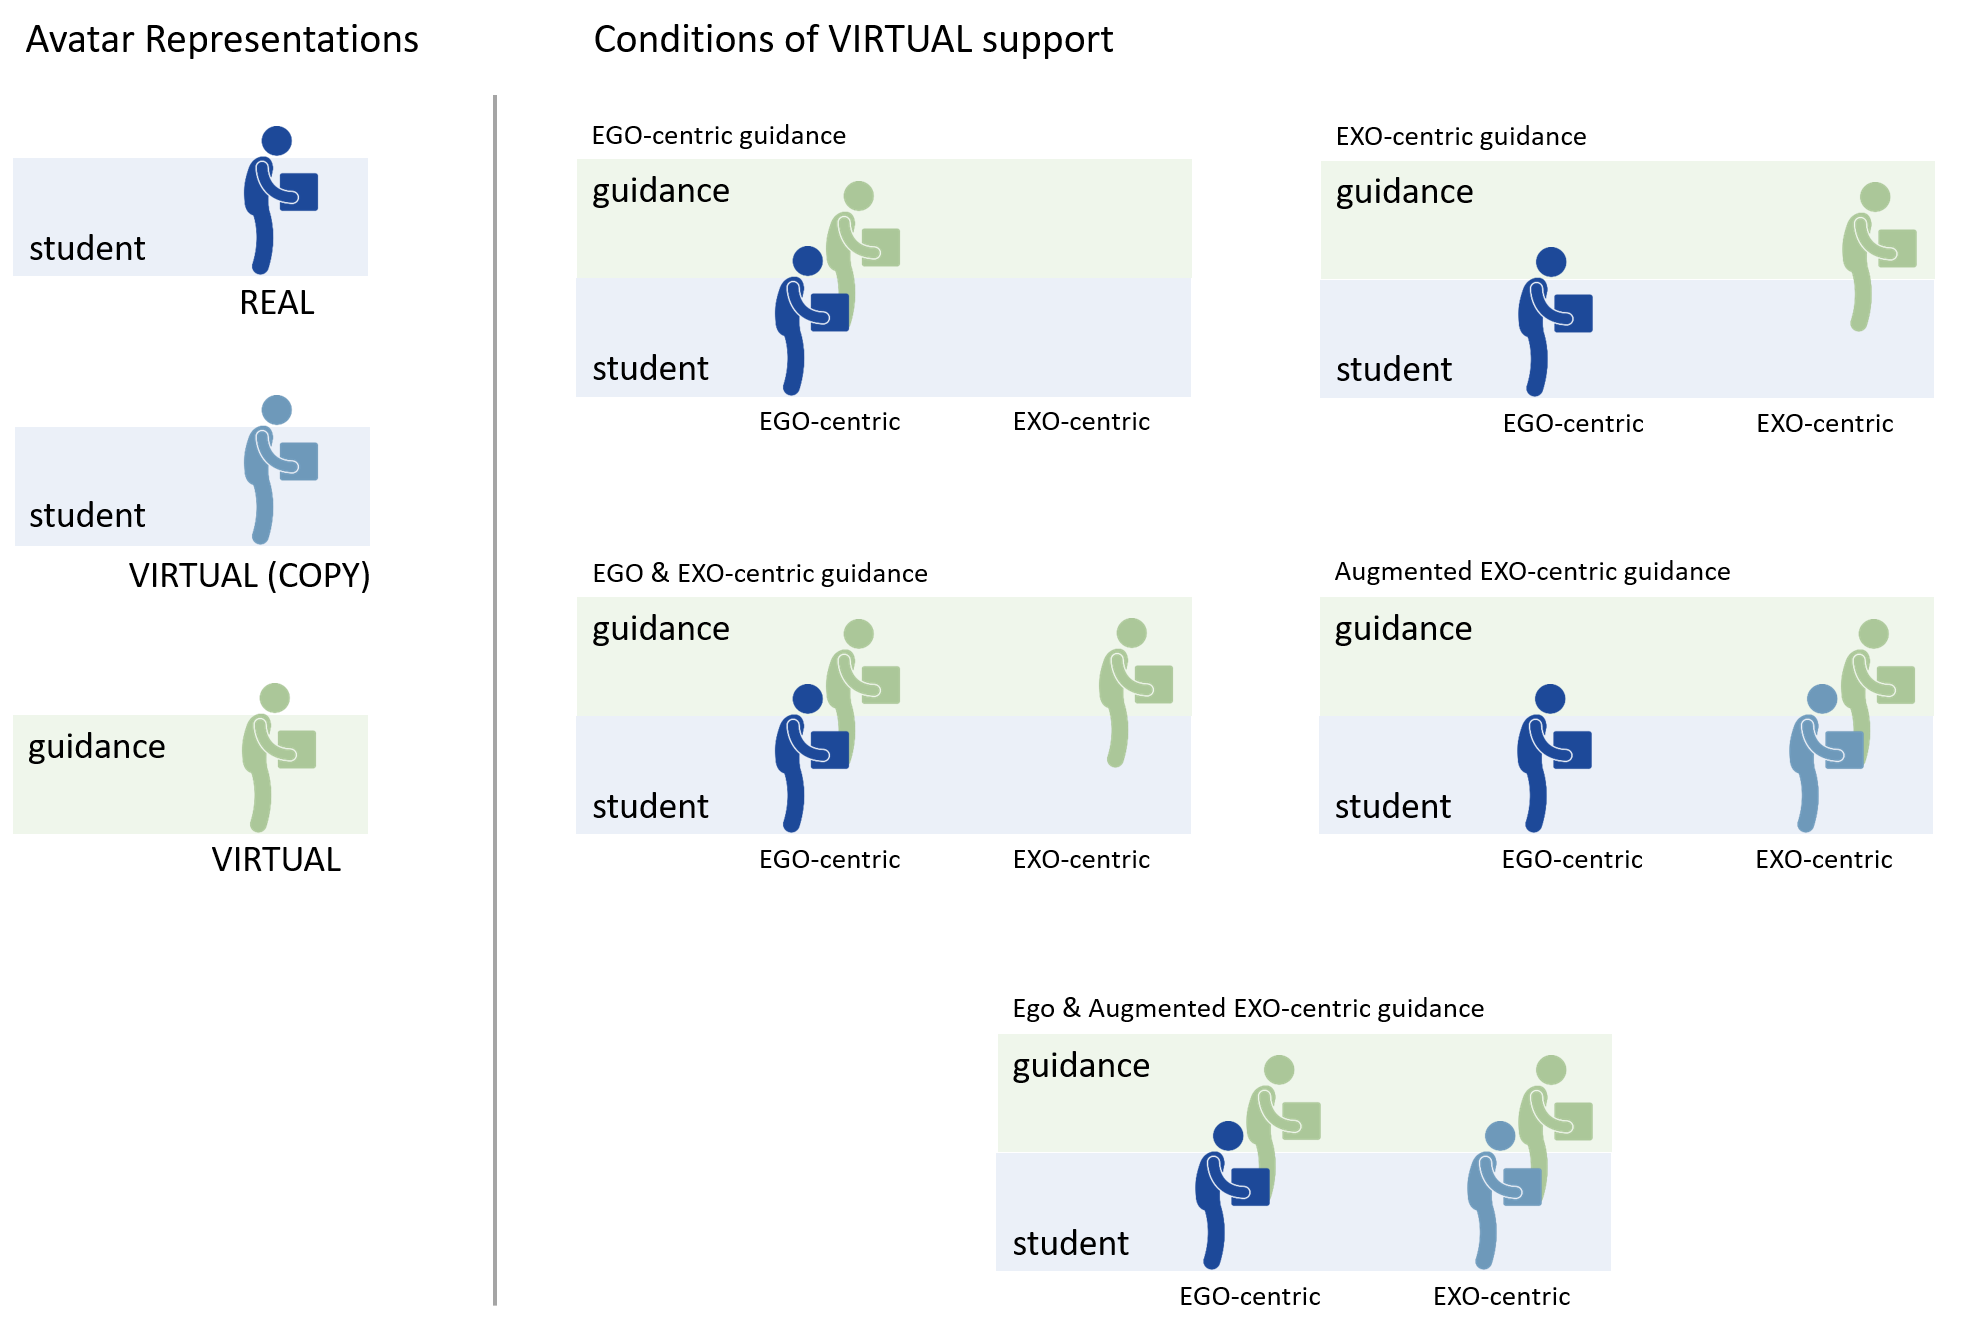
\includegraphics[width=\textwidth]{figures/perspectives.png}
	\caption[Possible perspectives]{Possible perspectives with one real world student and one real world teacher.}
	\label{fig:perspectives}
\end{figure}

\begin{figure}[htb]
	\centering
	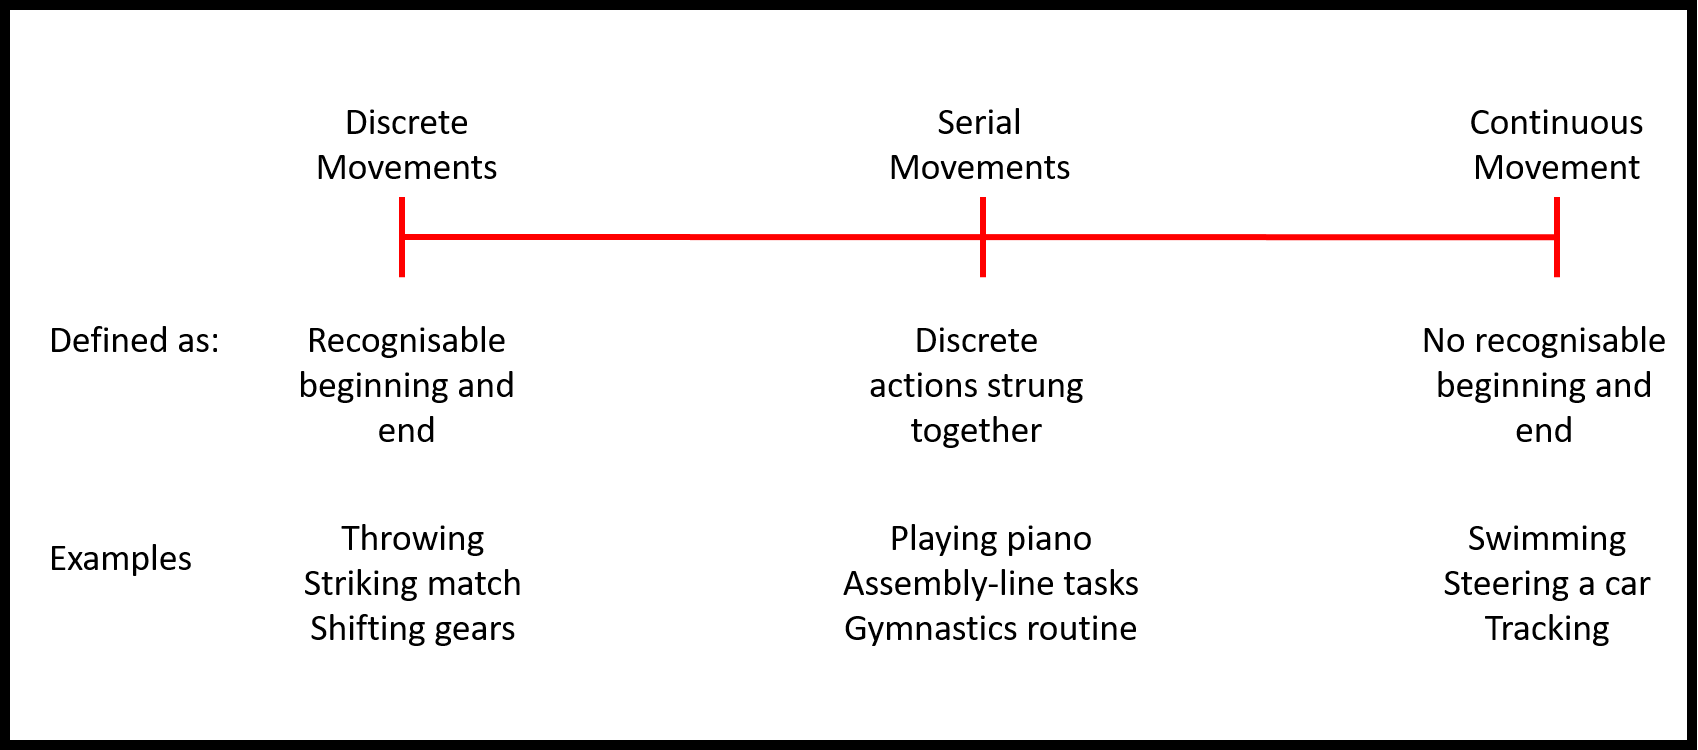
\includegraphics[width=\textwidth]{figures/movement_classification.png}
	\caption[Movement classification 1]{Movement classification 1}
	\label{fig:movement_classification}
\end{figure}

\begin{figure}[htb]
	\centering
	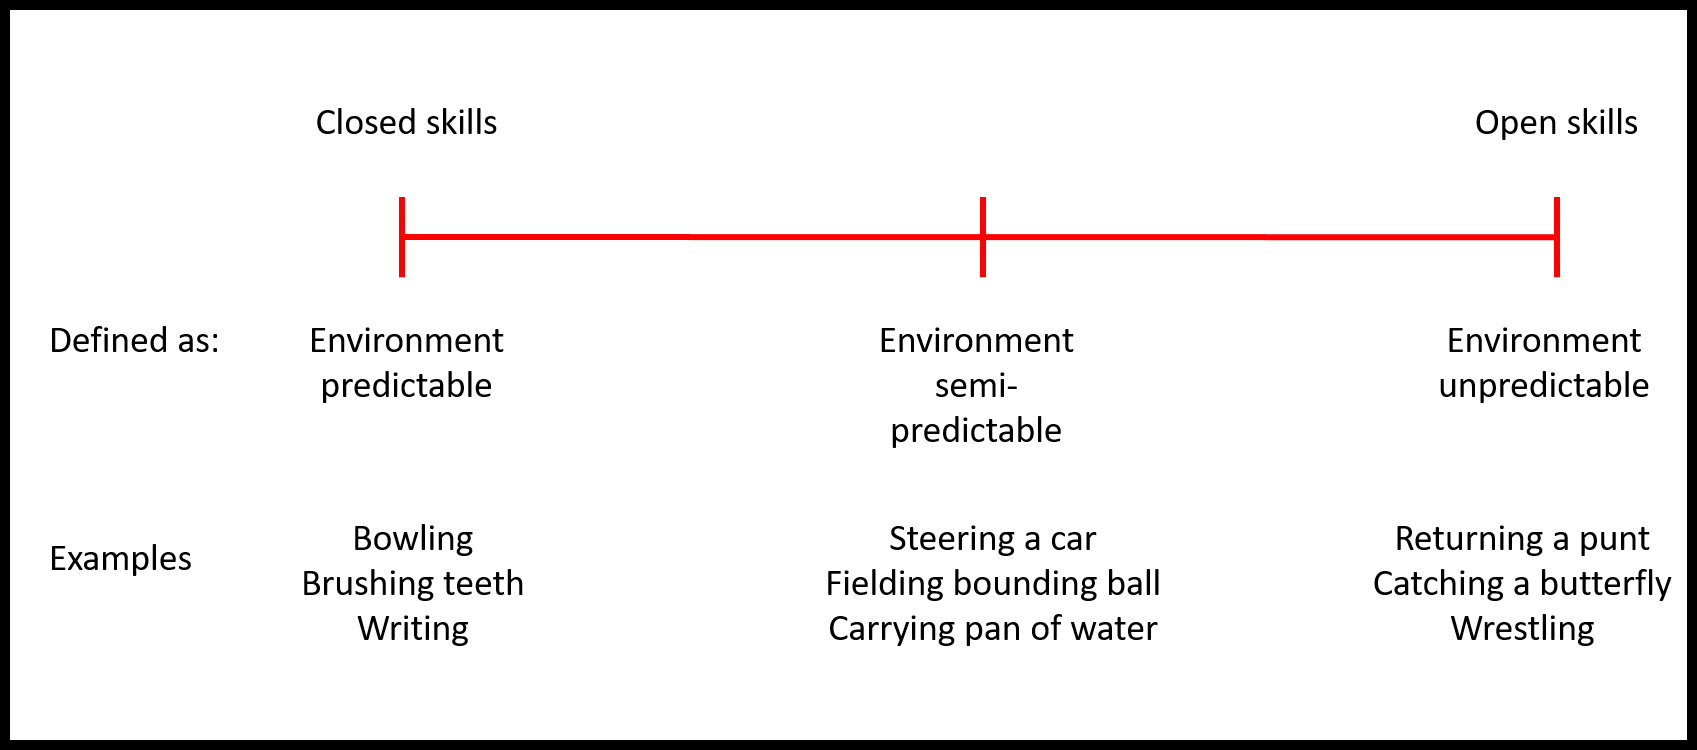
\includegraphics[width=\textwidth]{figures/movement_classification2.png}
	\caption[Movement classification 2]{Movement classification 2}
	\label{fig:movement_classification2}
\end{figure}

ego-exo continuum,
\subsection{measurements for motorlearning?}
\section{Handling Physical Load}
manual material handling~\cite{mmh}, single: lift lower push pull carry hold, hold out because of confusion with speed mechanic, introduced carry because of variaation and flexibility in task. unit/combined mmh tasks classification.\\
baua classification?
https://www.baua.de/EN/Topics/Work-design/Physical-workload/Types-of-workload/Types-of-workload_node.html https://www.baua.de/DE/Themen/Arbeitsgestaltung-im-Betrieb/Gefaehrdungsbeurteilung/Expertenwissen/Physische-Belastung/Heben-Halten-Tragen/Heben-Halten-Tragen_node.html
\section{Mixed Reality}
\label{section:mixed_reality}
\begin{figure}[htb]
	\centering
	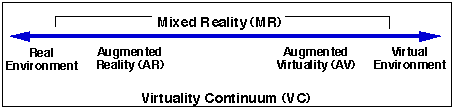
\includegraphics[width=\textwidth]{figures/milgram_continuum.png}
	\caption[Ego-Exo continuum by Milgram]{Ego-centric / exo-centric continuum by Milgram \todo{source}}
	\label{fig:mr_continuum}
\end{figure}


argumentation warum VR und nicht AR?
\section{Related Work: Motor Learning in Virtual Reality}
Similar setup~\cite{samesetup}
\label{section:related_work}
\begin{figure}[htb]
	\centering
	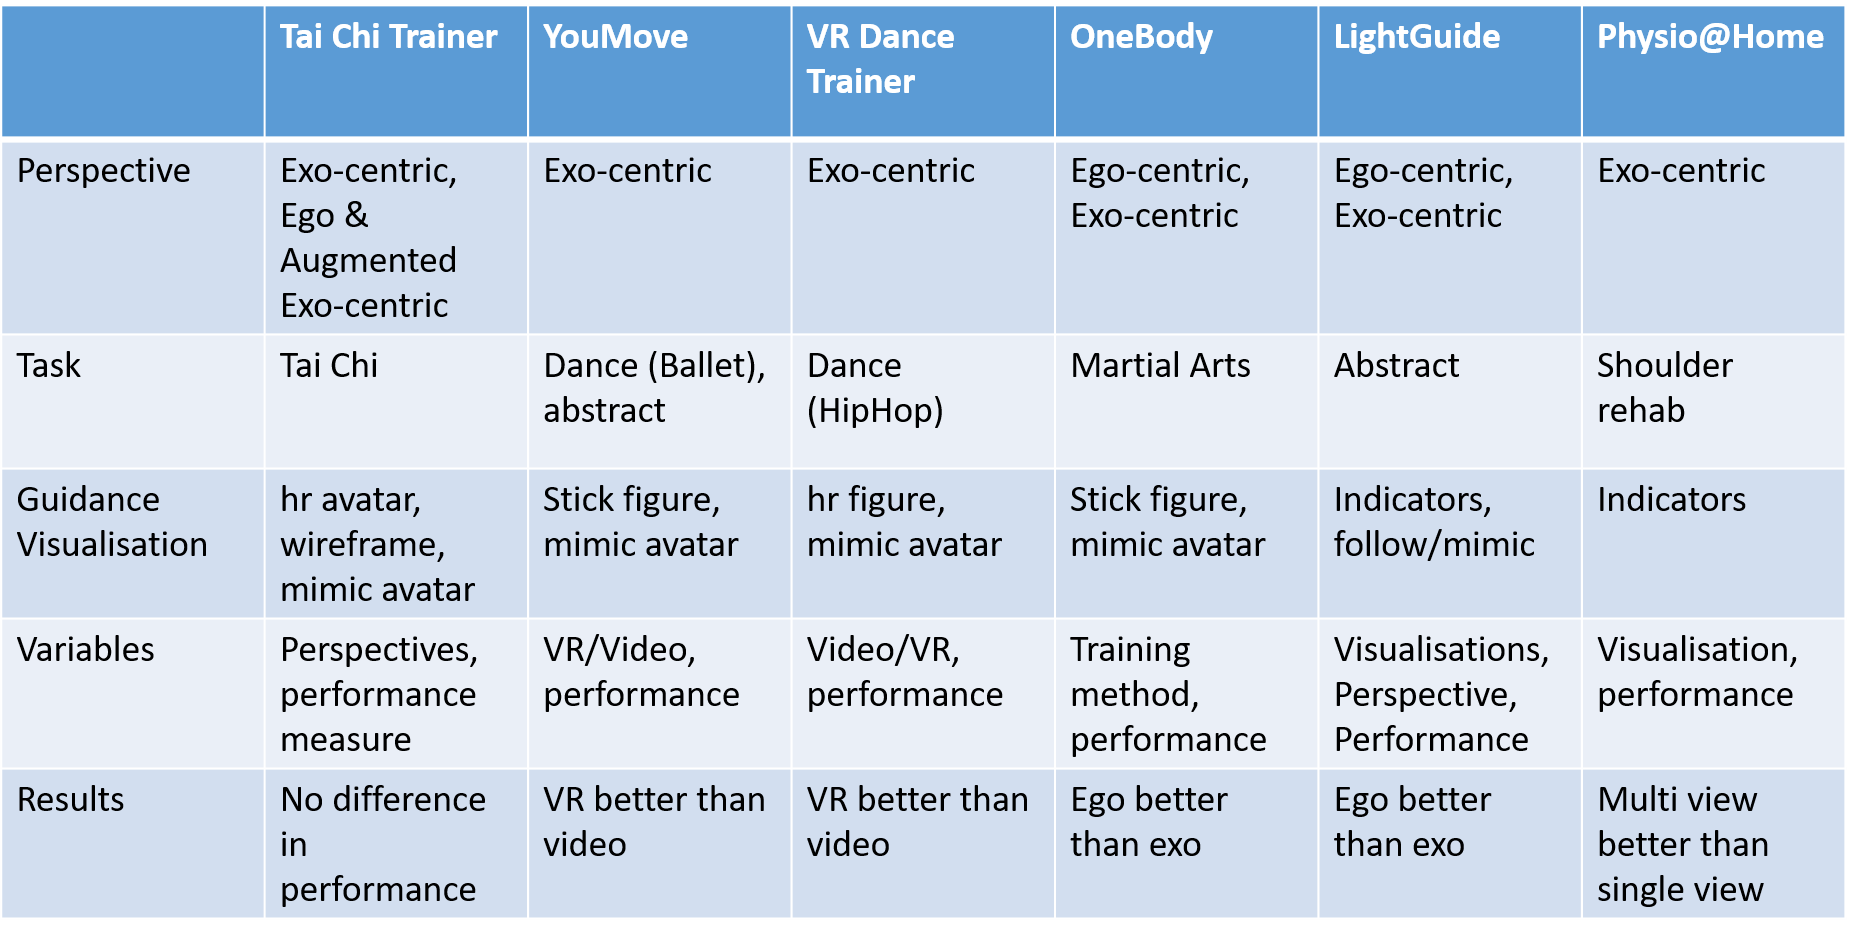
\includegraphics[width=\textwidth]{figures/detail_paper_overview.png}
	\caption[Overview seminar evaluation]{Overview seminar evaluation}
	\label{fig:rw_overview_detail}
\end{figure}

\begin{figure}[htb]
	\centering
	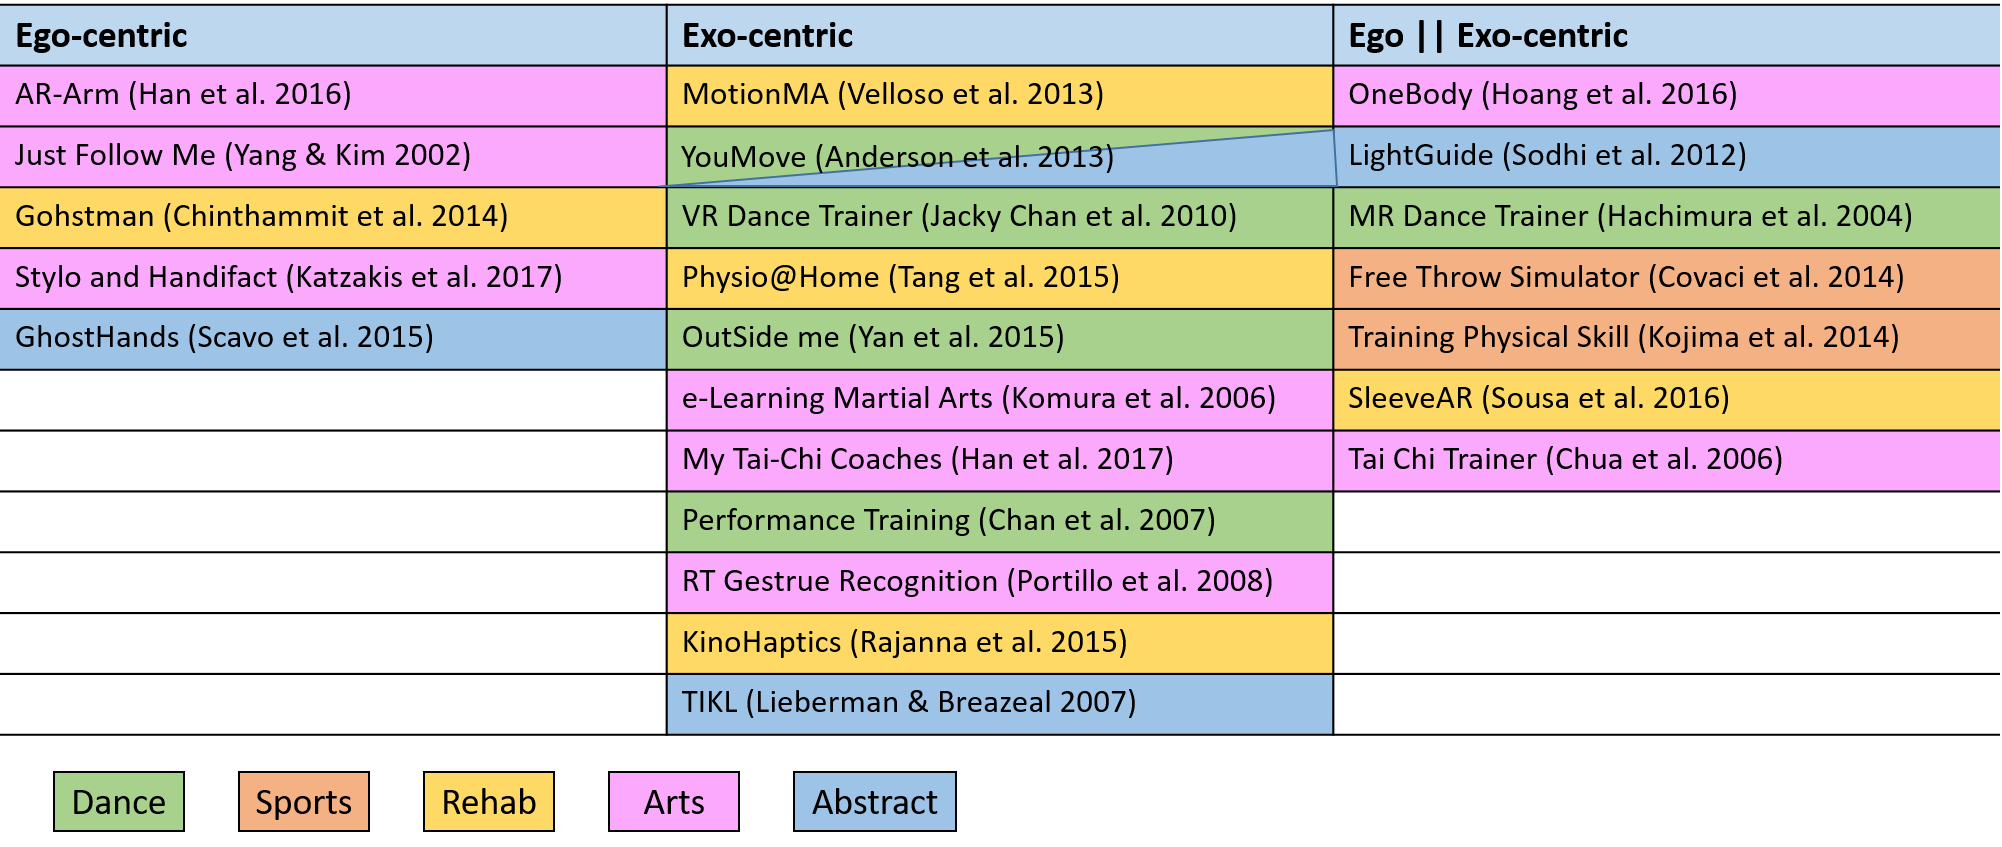
\includegraphics[width=\textwidth]{figures/rw_overview.png}
	\caption[Overview seminar evaluation]{Overview Related Work divided by perspective and task}
	\label{fig:rw_overview}
\end{figure}
\section{Research Contribution Statement}
\label{delimination_contribution}
bekannte arbeiten und deren ergebnisse über motor learning in VR\\
\\
auf basis dieses kapitels wird die studie geformt

